\chapter{Einleitung}
Künstliche Intelligenz (KI) hat sich in den letzten Jahrzehnten zu einer der wichtigsten Technologien mit grossem Einfluss auf unser tägliches Leben entwickelt. Künstliche Intelligenz hat viele Anwendungen gefunden, die sowohl Chancen als auch Herausforderungen bieten, von der Medizin bis zur Wirtschaft. Dieser Text untersucht die Definition von künstlicher Intelligenz, ihre Entstehung und Verwendung im Alltag und untersucht die ethischen Fragen im Zusammenhang mit ihrer Verwendung.
\section{Definition der KI}
Künstliche Intelligenz bezeichnet die Fähigkeit von Computern und Maschinen, menschliche Aufgaben auszuführen, die normalerweise menschliche Intelligenz erfordern. Dabei geht es um Problemlösung, Lernen, Mustererkennung und Entscheidungsfindung. Algorithmen der künstlichen Intelligenz nutzen große Datenmengen und komplexe Modelle, um Muster zu erkennen und Vorhersagen zu treffen.
 
\begin{figure}[h]
    \centering
    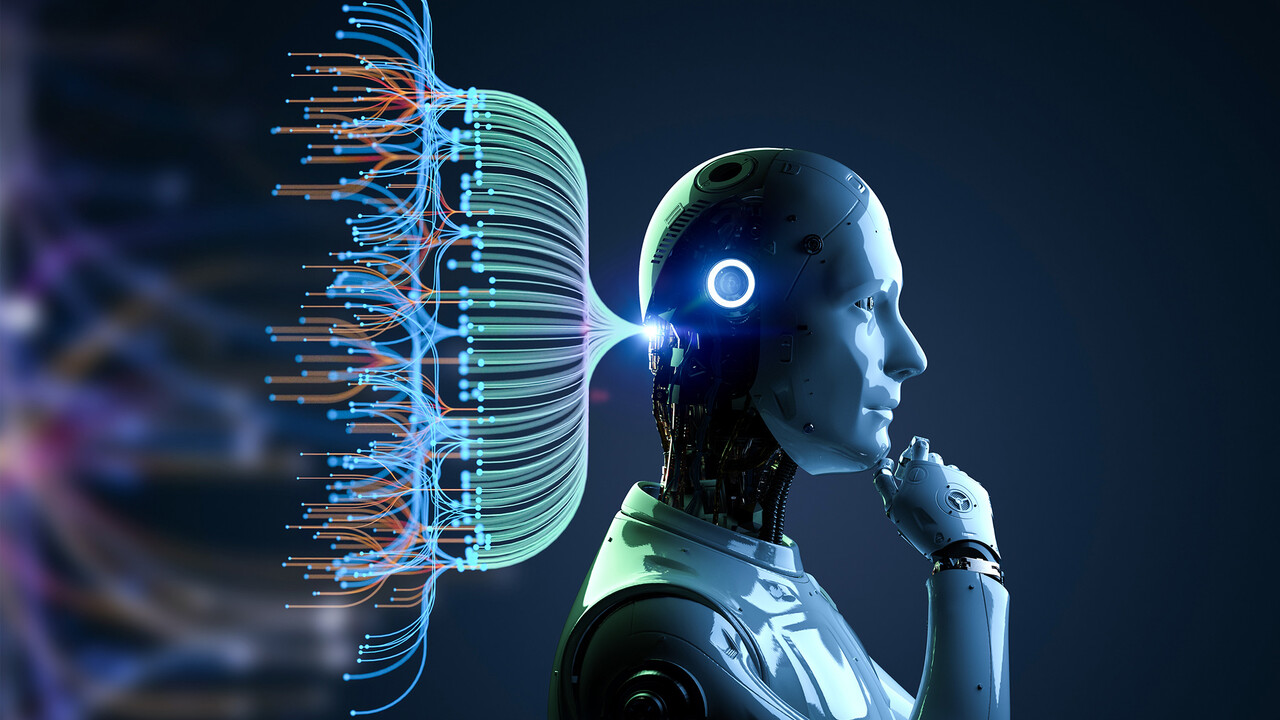
\includegraphics[width=0.5\textwidth]{KI.jpg}
    \caption{Künstliche Intelligenz}
    \label{fig:ai1}
\end{figure}